\chapter{面向过程}

\section{面向过程与面向对象}

\subsection{面向过程(Procedure Oriented)}

面向过程是一种以过程为中心的编程思想,以什么正在发生为主要目标进行编程,分析出解决问题所需要的步骤,然后用函数把这些步骤一步一步实现,使用的时候一个一个依次调用。\\

C语言就是一种面向过程的编程语言,但是面向过程的缺陷是数据和函数并不完全独立,使用两个不同的实体表示信息及其操作。\\

\subsection{面向对象(Object Oriented)}

面向对象是相对于面向过程来讲的,面向对象方法把相关的数据和方法组织为一个整体来看待,从更高的层次来进行系统建模,更贴近事物的自然运行模式。\\

在面向对象中,把构成问题的事物分解成各个对象,建立对象的目的不是为了完成一个步骤,而是为了描叙某个事物在整个解决问题的步骤中的行为。\\

Java、C++、Python等都是面向对象的编程语言,面向对象的优势在于只是用一个实体就能同时表示信息及其操作。\\

面向对象三大特性:

\begin{enumerate}
	\item 封装(encapsulation):数据和代码捆绑,避免外界干扰和不确定性访问。
	\item 继承(inheritance):让某种类型对象获得另一类型对象的属性和方法。
	\item 多态(polymorphism):同一事物表现出不同事物的能力。
\end{enumerate}

\newpage

\section{类与对象}

\subsection{类与对象}

类(class)表示同一类具有相同特征和行为的对象的集合,类定义了对象的属性和方法。\\

对象(object)是类的实例,对象拥有属性和方法。\\

类的设计需要使用关键字class,类名是一个标识符,遵循大驼峰命名法。类中可以包含属性和方法。其中,属性通过变量表示,又称实例变量;方法用于描述行为,又称实例方法。\\

在程序之中如果需要使用类,那么一般都会通过对象来进行操作。

\vspace{-0.5cm}

\begin{lstlisting}[language=Python]
obj_name = class_name([param])
\end{lstlisting}

当实例化了一个对象之后,就可以通过此对象进行类中成员的访问:

\begin{itemize}
	\item 对象.属性:访问类中的属性内容,如果程序中访问了没有定义的实例属性,那么将引发AttributeError异常。

	\item 对象.方法():调用类中的方法。对于类中每一个方法的当前对象都会有Python自己来负责该对象的传入,这一操作不是由用户负责的。
\end{itemize}

\vspace{0.5cm}

\mybox{类和对象}

\begin{lstlisting}[language=Python]
class Person:
    name = ""
    age = 0
    gender = ""

    def eat(self):
        print("吃饭")
    
    def sleep(self):
        print("睡觉")

def main():
    person = Person()
    
    person.name = "小灰"
    person.age = 16
    person.gender = "男"
    
    print("姓名:%s,年龄:%d,性别:%s" % (
            person.name, person.age, person.gender))
    person.eat()
    person.sleep()

if __name__ == "__main__":
    main()
\end{lstlisting}

\begin{tcolorbox}
	\mybox{运行结果}
	\begin{verbatim}
姓名:小灰,年龄:16,性别:男
吃饭
睡觉
\end{verbatim}
\end{tcolorbox}

\vspace{0.5cm}

\subsection{垃圾回收机制}

引用传递的本质在于将同一块空间修改权力交由不同的对象来完成,在这样的处理之中就有可能产生垃圾空间。在Python的引用数据处理之中都会存在有一个引用计数器,当引用计数器为0的时候就表示该对象已经成为了垃圾,等待进行回收。\\

\mybox{垃圾回收机制}

\begin{lstlisting}[language=Python]
class Person:
    pass

def main():
    person1 = Person()
    person2 = Person()

    print("【引用传递前地址】person1: %d, person2: %d" % (
            id(person1), id(person2)))
    person2 = person1
    print("【引用传递后地址】person1: %d, person2: %d" % (
            id(person1), id(person2)))

if __name__ == "__main__":
    main()
\end{lstlisting}

\begin{tcolorbox}
	\mybox{运行结果}
	\begin{verbatim}
【引用传递前地址】person1: 1988221852552, person2: 1988222686536
【引用传递后地址】person1: 1988221852552, person2: 1988221852552
\end{verbatim}
\end{tcolorbox}

在开发之中,实际上对于垃圾空间应该尽可能少的产生,虽然Python提供有垃圾收集机制,但是垃圾的回收与释放依然需要占用系统资源。

\newpage

\section{封装}

\subsection{封装(Encapsulation)}

封装是面向对象方法的重要原则,就是把对象的属性和方法结合为一个独立的整体,并尽可能隐藏对象的内部实现细节。\\

封装可以认为是一个保护屏障,防止该类的数据被外部类随意访问。要访问该类的数据,必须通过严格的接口控制。合适的封装可以让代码更容易理解和维护,也加强了程序的安全性。\\

实现封装的步骤:

\begin{enumerate}
	\item 修改属性的可见性来限制对属性的访问,一般限制为private。
	\item 对每个属性提供对外的公共方法访问,也就是提供一对setter / getter,用于对私有属性的访问。
\end{enumerate}

\vspace{0.5cm}

\mybox{封装}

\begin{lstlisting}[language=Python]
class Person:
    def set_name(self, name):
        self.__name = name
    
    def get_name(self):
        return self.__name
    
    def set_age(self, age):
        self.__age = age
    
    def get_age(self):
        return self.__age

def main():
    person = Person()
    person.set_name("小灰")
    person.set_age(17)
    print("姓名:%s,年龄:%d" % (
            person.get_name(), person.get_age()))

if __name__ == "__main__":
    main()
\end{lstlisting}

\begin{tcolorbox}
	\mybox{运行结果}
	\begin{verbatim}
姓名:小灰,年龄:17
\end{verbatim}
\end{tcolorbox}

\newpage

\section{构造方法与析构方法}

\subsection{构造方法(Constructor)}

构造方法也是一个方法,用于实例化对象,在实例化对象的时候调用。一般情况下,使用构造方法是为了在实例化对象的同时,给一些属性进行初始化赋值。\\

构造方法和普通方法的区别:

\begin{enumerate}
	\item 构造方法的名称必须为\_\_init\_\_()。
	\item 构造方法没有返回值。
	\item 一个类中只允许定义最多1个构造方法。
\end{enumerate}

如果一个类中没有写构造方法,系统会自动提供一个无参构造方法,以便实例化对象。\\

\mybox{构造方法}

\begin{lstlisting}[language=Python]
class Person:
    def __init__(self, name, age):
        self.__name = name
        self.__age = age
    
    def get_info(self):
        return "姓名:%s,年龄:%d" % (self.__name, self.__age)

def main():
    person = Person("小灰", 17)
    print(person.get_info())

if __name__ == "__main__":
    main()
\end{lstlisting}

\begin{tcolorbox}
	\mybox{运行结果}
	\begin{verbatim}
姓名:小灰,年龄:17
\end{verbatim}
\end{tcolorbox}

\vspace{0.5cm}

\subsection{析构方法(Destructor)}

在对象实例化的时候会触发构造方法的执行,与之对应的操作称为析构,当对象不再使用的时候进行某些收尾处理的操作。析构方法名称也要要求,必须为\_\_del\_\_()。\\

\mybox{析构方法}

\begin{lstlisting}[language=Python]
class Person:
    def __init__(self):
        print("构造方法被执行了")
    
    def __del__(self):
        print("析构方法被执行了")

def main():
    person = Person()
    del person

if __name__ == "__main__":
    main()
\end{lstlisting}

\begin{tcolorbox}
	\mybox{运行结果}
	\begin{verbatim}
构造方法被执行了
析构方法被执行了
\end{verbatim}
\end{tcolorbox}

\vspace{0.5cm}

\subsection{匿名对象}

对象的名称只是一个地址的信息,真正的内容是保存在内存中的,如果不需要名称就可以使用匿名对象。匿名对象使用完成之后由于没有其它对象进行引用,那么就有可能被垃圾回收,同时也会调用析构方法。\\

如果一个对象要被反复使用,那么可以定义有名对象;如果一个对象只是用一次,就采用匿名对象完成操作即可。\\

\mybox{匿名对象}

\begin{lstlisting}[language=Python]
class Person:
    def __init__(self, name, age):
        self.__name = name
        self.__age = age
    
    def get_info(self):
        return "姓名:%s,年龄:%d" % (self.__name, self.__age)

def main():
    print(Person("小灰", 17).get_info())

if __name__ == "__main__":
    main()
\end{lstlisting}

\begin{tcolorbox}
	\mybox{运行结果}
	\begin{verbatim}
姓名:小灰,年龄:17
\end{verbatim}
\end{tcolorbox}

\newpage

\section{继承}

\subsection{继承(Inheritance)}

继承是面向对象的三大特征之一,程序中的继承是类与类之间的特征和行为的一种赠予或获取。两个类之间的继承必须满足“is a”的关系。子类继承自父类,父类也称基类或超类,子类也称派生类。

\begin{figure}[H]
	\centering
	\begin{tikzpicture}
		\begin{class}{Animal}{0,0}
			\attribute{- age}
			\attribute{- gender}
			\operation{+ eat() : void}
			\operation{+ sleep() : void}
		\end{class}

		\begin{class}{Dog}{-5,-5}
			\inherit{Animal}
			\attribute{- type}
			\operation{+ bite() : void}
		\end{class}

		\begin{class}{Cat}{5,-5}
			\inherit{Animal}
			\attribute{- hairColor}
			\operation{+ mewing() : void}
		\end{class}
	\end{tikzpicture}
	\caption{继承}
\end{figure}

产生继承关系后,子类可以使用父类中的属性和方法,也可以定义子类独有的属性和方法。

\vspace{-0.5cm}

\begin{lstlisting}[language=Python]
class subclass(superclass1, ...):
    # code
\end{lstlisting}

在进行继承的时候,子类会继承父类之中全部定义的结构。但是对于构造方法的继承是比较特殊的,需要考虑两种情况:

\begin{enumerate}
	\item 当父类定义了构造方法,但是子类没有定义构造方法时,实例化子类对象会自动调用父类中提供的无参构造方法。

	\item 当子类定义了构造方法时,将不再默认调用父类中的任何构造方法,但是可以手动调用。如果有需要也可以通过super类的实例实现子类调用父类结构的需求。
\end{enumerate}

\vspace{0.5cm}

\mybox{继承}

\begin{lstlisting}[language=Python]
class Animal:
    def __init__(self, name, age):
        self.__name = name
        self.__age = age
    
    def set_name(self, name):
        self.__name = name

    def get_name(self):
        return self.__name
    
    def set_age(self, age):
        self.__age = age

    def get_age(self):
        return self.__age

    def eat(self):
        print("吃饭")
    
    def sleep(self):
        print("睡觉")
    
class Dog(Animal):
    def __init__(self, name, age, type):
        super().__init__(name, age)
        self.__type = type
    
    def set_type(self, type):
        self.__type = type

    def get_type(self):
        return self.__type
    
    def bite(self):
        print("咬人")

def main():
    dog = Dog("狗子", 3, "哈士奇")
    
    print("姓名:%s,年龄:%d,品种:%s" % (
            dog.get_name(), dog.get_age(), dog.get_type()))

    dog.eat()
    dog.sleep()
    dog.bite()

if __name__ == "__main__":
    main()
\end{lstlisting}

\begin{tcolorbox}
	\mybox{运行结果}
	\begin{verbatim}
姓名:狗子,年龄:3,品种:哈士奇
吃饭
睡觉
咬人
\end{verbatim}
\end{tcolorbox}

\vspace{0.5cm}

\subsection{多继承}

多继承指一个子类可以同时继承多个父类的内容,在多继承实现中只需要编写多个父类的名称即可。\\

利用多继承的最大优势在于可以在进行子类操作的时候将多个父类中定义的结构全部保留继续使用。\\

\mybox{多继承}

\begin{lstlisting}[language=Python]
class Date:
    def set_date(self, year=1970, month=1, day=1):
        self.__year = year
        self.__month = month
        self.__day = day
    
    def get_date(self):
        return "%04d/%02d/%02d" % (
            self.__year, self.__month, self.__day)
    
class Time:
    def set_time(self, hour=0, minute=0, second=0):
        self.__hour = hour
        self.__minute = minute
        self.__second = second
    
    def get_time(self):
        return "%02d:%02d:%02d" % (
            self.__hour, self.__minute, self.__second)

class DateTime(Date, Time):
    def __init__(self, year=1970, month=1, day=1, 
                       hour=0, minute=0, second=0):
        super().set_date(year, month, day)
        super().set_time(hour, minute, second)
    
    def __repr__(self):
        return super().get_date() + " " + super().get_time()

def main():
    date_time = DateTime(2021, 4, 6, 14, 38, 40)
    print(date_time)

if __name__ == "__main__":
    main()
\end{lstlisting}

\begin{tcolorbox}
	\mybox{运行结果}
	\begin{verbatim}
2021/04/06 14:38:40
\end{verbatim}
\end{tcolorbox}

\newpage

\section{多态}

\subsection{多态(Polymorphism)}

多态是同一个行为具有多个不同表现形式或形态的能力。

\begin{figure}[H]
	\centering
	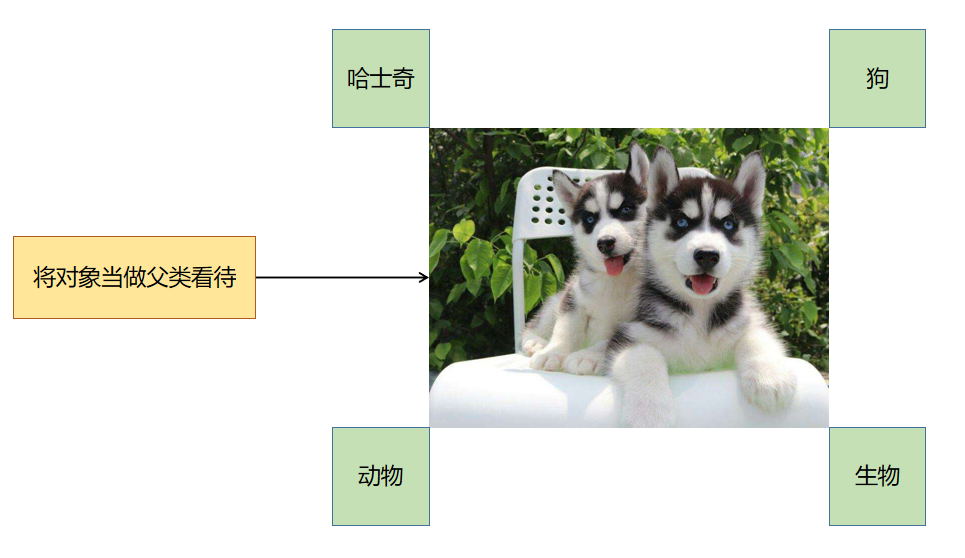
\includegraphics[scale=0.7]{img/C7/7-6/1.png}
	\caption{多态}
\end{figure}

在类继承的结构之中,很难保证父类中的某些操作方法可以被子类继续拿来使用。这个时候子类为保留住原始的方法名称,同时也为了可以对功能实现进一步的扩充,就可以利用方法覆写。\\

\mybox{多态}

\begin{lstlisting}[language=Python]
import math

class Shape:
    def get_area(self):
        pass

class Rectangle(Shape):
    def __init__(self, width, length):
        self.__width = width
        self.__length = length
    
    def get_area(self):
        return self.__length * self.__width

class Circle(Shape):
    def __init__(self, radius):
        self.__radius = radius
    
    def get_area(self):
        return math.pi * self.__radius ** 2

def shape_area(obj):
    if isinstance(obj, Shape):
        return obj.get_area()

def main():
    print("长方形面积:%.2f" % shape_area(Rectangle(6, 11)))
    print("圆形面积:%.2f" % shape_area(Circle(5)))

if __name__ == "__main__":
    main()
\end{lstlisting}

\begin{tcolorbox}
	\mybox{运行结果}
	\begin{verbatim}
长方形面积:66.00
圆形面积:78.54
\end{verbatim}
\end{tcolorbox}

\newpage